\documentclass[11pt,a4paper]{article}
\usepackage[margin=2.2cm]{geometry}
\usepackage[T1]{fontenc}
\usepackage{lmodern}
\usepackage{microtype}
\usepackage{booktabs}
\usepackage{tabularx}
\usepackage{graphicx}
\usepackage{enumitem}
\usepackage{xcolor}
\usepackage[hidelinks]{hyperref}
\usepackage{amsmath}

\setlist{itemsep=2pt,topsep=4pt}
\newcommand{\src}[1]{\texttt{\small #1}}
\newcommand{\dec}[1]{\textsf{#1}}

\title{Robotic Ultrasound with Soft Tissue: Progress Report\\[2pt]
\large 5--12 November 2026, including the MuJoCo soft-body attempt}
\author{MTP project}
\date{12 November 2026}

\begin{document}
\maketitle

\noindent Every number in this report comes from a file in \src{results/}, a test, or a \dec{DEC} entry in
\src{DECISIONS.md} that names its source. The source sits next to each table. All runs are on the laptop
(i5-1240P, RTX~2050, 4~GB); the workstation GPU was not reachable this week.

\section*{Summary}
\begin{itemize}
  \item \textbf{Goal (confirmed 12 Nov).} SonoGym's tasks with patient-specific soft-tissue deformation added, and
    \emph{findings} about what the deformation changes for a robot scanning with ultrasound.
  \item \textbf{The gym exists.} \src{mtp\_gym} runs SonoGym's 12 patients plus one, on a GPU-batched linear FEM,
    with force control and B-mode rendered from the deformed CT (\dec{DEC-041}).
  \item \textbf{No task has yet shown that deformation changes an outcome.} Three attempts this week found that it did
    not matter or could not be measured (\dec{DEC-048}, \dec{DEC-051}). This is the main open problem.
  \item \textbf{MuJoCo (10--12 Nov).} As a rigid-body backend it works: it holds 1~kHz and gives a compliant,
    torque-controlled robot. As a soft-tissue model it \textbf{failed a pre-registered gate} against a
    finite-strain reference. One material is wrong from first contact; the other is accurate at low force but
    about 380 times over the 33~ms time budget (\dec{DEC-053}). MuJoCo flex therefore stays demo only.
  \item \textbf{The failure costs the paper little.} The gym never needed MuJoCo, and the project's FEM is within
    5\,\% of the reference at the working force (\dec{DEC-047}).
  \item \textbf{RSS 2027 Stage 1 abstract due 4 December}: 22 days.
\end{itemize}

%=====================================================================================================
\section{Work on the gym and the studies (5--8 November)}

\subsection{What was built}
\begin{itemize}
  \item \textbf{GPU-batched gym} (\dec{DEC-041}). Gymnasium \texttt{VectorEnv} with the precomputed linear FEM solved
    for all environments in one batch. Four tasks:
    \begin{itemize}
      \item free scan;
      \item reconstruction (SonoGym task 2 analogue);
      \item navigation to the L4 plane (SonoGym task 1 analogue);
      \item force-commanded scan, which only makes sense with soft tissue.
    \end{itemize}
  \item \textbf{Patients.} 13 in total: the 12 TotalSegmentator subjects SonoGym uses, plus the sample patient. The
    split is 9 train and 4 held out, stratified by tissue thickness. All patients share the same tissue moduli.
  \item \textbf{B-mode depth physics} (\dec{DEC-042}, \dec{DEC-043}): per-tissue attenuation, receiver noise and a
    fixed TGC.
  \item \textbf{Benchmark-validity fixes.}
    \begin{itemize}
      \item A hidden patient-placement offset, because a blind policy solved navigation from the pose alone
        (\dec{DEC-045}).
      \item A coverage-gain reward, because the area reward paid for wandering (\dec{DEC-046}).
    \end{itemize}
  \item \textbf{A Neo-Hookean finite-strain reference FEM}, to check the linear FEM (\dec{DEC-047}).
\end{itemize}

\subsection{Results}
\begin{table}[h]
\centering\small
\begin{tabularx}{\linewidth}{@{}lXl@{}}
\toprule
Study & Result & Source \\
\midrule
FEM fidelity & Linear vs Neo-Hookean compression: median $-1.3\,\%$ (range $-4.9$ to $+1.8$) at 2~N; up to about
  $\pm 30\,\%$ at 5--15~N. Accurate only at low force. & \src{fem\_fidelity\_20261107\_234638} \\
Depth physics & Mean coverage over 13 patients 0.659 (legacy) $\to$ 0.376; it falls with paraspinal fat
  (Spearman $\rho=-0.79$). & \src{bmode\_physics\_compare\_20261107\_190506} \\
H2: force vs image & \textbf{Pre-registered, failed.} The best force is 2~N for thin and thick backs alike. & \dec{DEC-042}, \dec{DEC-044} \\
Perception tuning & Held-out coverage 0.318 $\to$ 0.428 at precision 0.979. The two fattest backs stay at 0.01--0.07. & \src{perception\_tuning\_20261107\_190845} \\
Navigation PPO & 100\,\% success on its 2 training patients, 7.8\,\% on 4 held-out patients. & \src{vec\_eval\_nav\_20261107\_223741} \\
Echo shift (thread C) & The bone-echo shift under force is the same with and without the FEM warp: the deformation
  part is 0.00~mm in 11 of 12 patients. \textbf{The shift is probe kinematics}, and the earlier claim was withdrawn.
  & \src{kinematic\_vs\_deformation\_20261108\_020955} \\
Muscle thickness (thread B) & The muscle compresses (median 0.75~mm from 1 to 5~N), \textbf{but it cannot be measured
  from the image}: detection 0.38, error 7.3~mm. The CT-derived B-mode does not render the fascia. The gate failed.
  & \src{muscle\_compression\_20261108\_021028} \\
Generalisation (thread A) & Held-out navigation success is at most 14.1\,\% for every training set and augmentation
  (blind baseline 3.1\,\%). H1--H3 cannot be decided at laptop scale. & \src{vec\_eval\_nav\_20261108\_075931} \\
Reconstruction PPO & Does not beat random on held-out patients (0.32--0.34 vs 0.34; raster 0.43). & \src{vec\_eval\_recon\_20261108\_020410} \\
\bottomrule
\end{tabularx}
\caption{Results produced 5--8 November. Each source is a file in \src{results/} (\src{.md} and \src{.json}).}
\end{table}

\paragraph{Re-aim (\dec{DEC-048}, 8 Nov).} A hard self-review found the original central claim weak. With a tracked
probe, reconstruction of a rigid bone target is correct whether or not the tissue deforms (coverage 88.0 vs
88.8\,\%). The paper was re-aimed at two threads:
\begin{itemize}
  \item \textbf{Thread A:} cross-patient generalisation, with FEM-based augmentation as the novel arm.
  \item \textbf{Thread B:} a soft target whose measured size changes under compression (paraspinal muscle).
\end{itemize}
The 8 Nov runs left both without a positive result (table above).

%=====================================================================================================
\section{The MuJoCo attempt (10--12 November)}

\subsection{Why MuJoCo}
MuJoCo 4.0.0 (released 6 Nov) advertises native soft bodies (\emph{flex}). The hope was to address four limitations
of the current simulator, all recorded in \src{DECISIONS.md}:
\begin{itemize}
  \item frictionless contact;
  \item a kinematic robot (PyBullet's arm moves by less than 1~\textmu m under a 30~N push);
  \item quasi-static tissue;
  \item the linear FEM's error above 5~N.
\end{itemize}
Before any code, the engine's limits were checked (\dec{DEC-052}):
\begin{itemize}
  \item MuJoCo 4 needs Python $\geq$ 3.11, while the project runs Python 3.10, so the soft-body code got a second
    environment (\src{.venv-mj4}).
  \item A scratch timing put a 4~mm tetrahedral slab at tens of milliseconds per step. A soft body therefore cannot
    run inside the 1~ms physics tick and has to run in its own process.
\end{itemize}
The user chose a staged plan: Stage~1, MuJoCo replaces PyBullet for the robot; Stage~2, MuJoCo flex becomes a
tissue model only if it passes a gate written down \emph{before} the study.

\subsection{Stage 1: MuJoCo as the rigid-body engine --- works}
\begin{itemize}
  \item \textbf{What was built.}
    \begin{itemize}
      \item An engine-free physics loop (\src{physics\_common.py}) with two backends behind one interface.
      \item The same Panda robot, frame and messages as before.
      \item Torque-level control
        $\tau = b(q,\dot q) + M(q)\,[K_p(q_d-q)+K_d(\dot q_d-\dot q)]$, clipped to the robot's effort limits.
      \item Contract tests that run against both engines (\src{test\_physics\_backends.py}).
    \end{itemize}
  \item \textbf{The robot is now compliant.} A 30~N push deflects the MuJoCo arm by about 1.08~mm; the PyBullet arm
    moves by less than 1~\textmu m (printed by the tests).
  \item \textbf{Tracking.} In a sweep that translates and tilts the probe, the worst end-effector error is
    3.11~mm with MuJoCo and 7.29~mm with PyBullet (\src{test\_tilting\_sweep\_is\_tracked}; one trajectory).
  \item \textbf{A code review found and fixed} (test first):
    \begin{itemize}
      \item an IK that stopped before converging;
      \item a following-error clamp that drove the arm into a torque-saturated oscillation;
      \item a missing orientation-error report;
      \item unvalidated fixture input;
      \item concave keep-out fixtures treated as their convex hull, now one thin prism per triangle;
      \item a pre-existing bug: the L4 vertebra mesh was stored in millimetres where metres were expected, so it was
        drawn about 1000 times too large.
    \end{itemize}
  \item \textbf{Rate} (table~\ref{tab:rate}). Both engines hold 1~kHz on a quiet machine. The backend refactor did
    not slow PyBullet.
\end{itemize}

\begin{table}[h]
\centering\small
\begin{tabular}{@{}lccc@{}}
\toprule
Configuration & Rate (3 runs) & Tick compute p99 & Overruns / $\sim$20{,}000 ticks \\
\midrule
MuJoCo & 1000.0 Hz in 3 of 3 & 0.548--0.811 ms & 3--10 \\
PyBullet & 1000.0 Hz in 3 of 3 & 0.554--0.706 ms & 2--12 \\
PyBullet before the refactor (\texttt{ec88541}) & 1000.0 Hz in 3 of 3 & 0.691--0.835 ms & 8--26 \\
\bottomrule
\end{tabular}
\caption{Physics rate, 20~s runs, interleaved; source \src{results/physics\_rate\_20261112\_125735\_idle\_post\_review.json}
(script \src{scripts/physics\_rate\_compare.py}). The ranges overlap, so the runs do not rank the engines.}
\label{tab:rate}
\end{table}

\subsection{Stage 2: MuJoCo flex as the tissue model --- failed the gate}

\paragraph{Method (\dec{DEC-053}, pre-registered in commit \texttt{c7a7c9f} before any patient case ran).}
\begin{itemize}
  \item \textbf{Cases:} the same as the FEM-fidelity study, i.e. 3 patients (sample, a thin back s0015, a thick back
    s0014) $\times$ 2 sites $\times$ 4 forces (2, 5, 10, 15~N).
  \item \textbf{Mesh:} the same 4~mm patient mesh, the same fixed nodes and the same fat/muscle moduli. Two material
    models: Saint Venant--Kirchhoff (SVK, MuJoCo's default) and MuJoCo's Stable Neo-Hookean.
  \item \textbf{Loading:} the same nodal forces were applied to the flex as to the reference, so only the material
    model is compared.
  \item \textbf{Reference:} the Neo-Hookean result of \dec{DEC-047}.
\end{itemize}
A material passes only if all four of these hold:
\begin{itemize}
  \item \textbf{G1}, every case within 10\,\% at 2--5~N;
  \item \textbf{G2}, a median error at 10--15~N no worse than the linear FEM's;
  \item \textbf{G3}, no inverted element;
  \item \textbf{G4}, a warm re-settle after a 0.33~mm step within 33~ms, or 100~ms as ``10~Hz tissue''.
\end{itemize}
One trick made heterogeneous tissue possible in a single flex: scaling each element's compiled stiffness gives
per-element moduli. A test asserts this, and it fails if the scaling is removed (G5).

\begin{table}[h]
\centering\small
\begin{tabularx}{\linewidth}{@{}lXXXXc@{}}
\toprule
Material & G1 (2--5~N) & G2 (10--15~N) & G3 (stability) & G4 (cost) & Passes \\
\midrule
SVK & fail (90--420\,\% too much compression at 2~N) & fail (median 252\,\% vs linear 15\,\%) & fail (inverted
  elements in all 24 cases, up to 6{,}409) & fail (50.5~s) & no \\
Stable Neo-Hookean & fail (one 5~N case at +15.1\,\%; 2~N within 1.2--4.5\,\%) & fail (median 18.8\,\% vs linear
  14.9\,\%) & fail (up to 39 inverted, 7 of 24 cases) & fail (12.5~s) & no \\
\bottomrule
\end{tabularx}
\caption{DEC-053 gate. Source \src{results/mujoco\_flex\_fidelity\_20261112\_112537.md}; 48 rows, 4 without a
reference (the Neo-Hookean solve itself did not converge there) excluded as pre-registered. All 48 flex cases
settled.}
\end{table}

\begin{figure}[h]
\centering
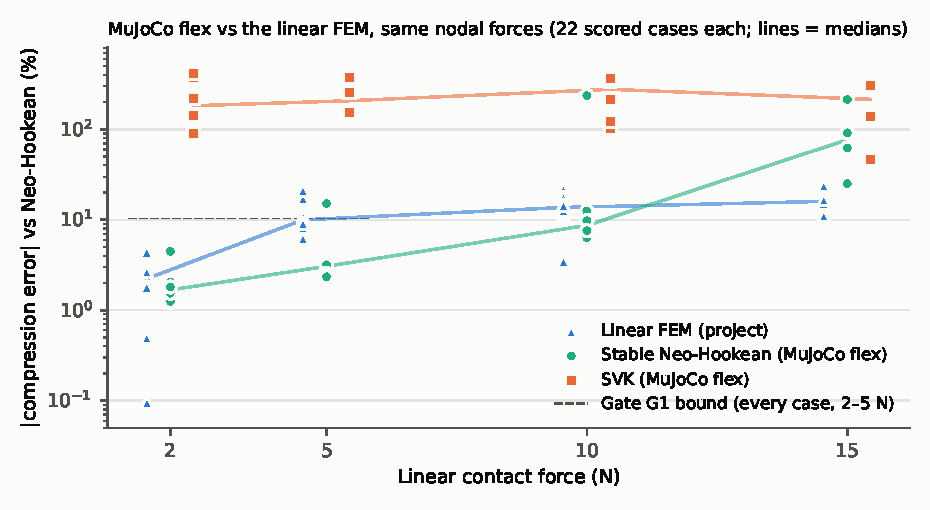
\includegraphics[width=0.92\linewidth]{fig_flex_gate.pdf}
\caption{Error in compression under the probe, relative to the Neo-Hookean reference, for each scored case
(log scale). Made by \src{make\_figures.py} from the same results file.}
\end{figure}

\subsection{Why it failed}
\begin{enumerate}
  \item \textbf{SVK is wrong from first contact.}
    \begin{itemize}
      \item Even at 2~N the elements under the loaded skin nodes are strongly compressed: the contact force acts on
        a few nodes.
      \item SVK is a material model known to lose stiffness under strong compression and to allow elements to turn
        inside out.
      \item Every SVK case has inverted elements, and its compression is 90--420\,\% too large.
      \item This cannot be fixed by staying at low force.
    \end{itemize}
  \item \textbf{Stable Neo-Hookean is close at low force and drifts at high force.}
    \begin{itemize}
      \item Its energy is not the same compressible Neo-Hookean energy as the reference. The two agree at small
        strain (2~N: within 4.5\,\%) and part ways at large strain.
      \item Above 10~N, 7 of 24 cases also invert some elements.
      \item We did not separate these two causes.
      \item At 2--5~N it would be usable; but there the project's linear FEM is already within about 5\,\%
        (\dec{DEC-047}), so it adds nothing.
    \end{itemize}
  \item \textbf{Cost is structural, not a tuning problem.}
    \begin{itemize}
      \item MuJoCo time-steps the whole mesh (15--25 thousand nodes) until it comes to rest: 98 steps and 12.5~s for
        one re-settle.
      \item The project's FEM precomputes the tissue's response once. Each query is then small dense algebra plus
        one GPU matrix--vector product, which fits the 30~Hz streaming loop.
      \item A dynamic solver cannot answer quasi-static queries at that speed, and a finer mesh would only be
        slower.
    \end{itemize}
\end{enumerate}
\noindent Ruled out as causes:
\begin{itemize}
  \item the per-element moduli (asserted by a test);
  \item failure to settle (all 48 cases settled);
  \item a units or setup error (the two materials agree at small load in
    \src{test\_both\_materials\_agree\_at\_small\_load\_and\_settle\_without\_inversion}).
\end{itemize}

\subsection{What remains from the MuJoCo work}
\begin{itemize}
  \item A second, tested physics backend with a compliant robot, concave fixtures and a corrected L4 mesh. It is on
    branch \src{mujoco-bridge}; PyBullet stays the default.
  \item \texttt{--tissue-backend mujoco-flex}: a live MuJoCo soft body pressed by the probe and streamed to 3D
    Slicer (\src{scripts/demo\_mujoco\_flex\_slicer.sh}).
    \begin{itemize}
      \item It is \textbf{demo only}: the gym and the benchmark reject it (tested).
      \item A trial run produced the renders and Slicer captures; no recording is committed yet.
    \end{itemize}
  \item A reportable negative result: ``an off-the-shelf soft-body engine is either inaccurate (SVK) or about
    380 times over the time budget (Stable Neo-Hookean) for interactive quasi-static tissue; a precomputed FEM is within
    5\,\% in the working range''.
  \item The robot's deflection is \emph{not} fed back into the tissue solve or the image. The caveat that the
    robot is kinematic therefore still applies to every reported result.
\end{itemize}

%=====================================================================================================
\section{Current status}

\begin{table}[h]
\centering\small
\begin{tabularx}{\linewidth}{@{}lX@{}}
\toprule
Branch & Contents \\
\midrule
\src{main} & Up to 7 Nov: gym, 13 patients, depth B-mode, the validity fixes, the navigation result (PR \#3). \\
\src{audit-fixes} & \src{main} plus 7--8 Nov: FEM fidelity, the \dec{DEC-048} re-aim, the thread A/B/C studies. Not merged. \\
\src{mujoco-bridge} & \src{audit-fixes} plus the MuJoCo work, both gates, this report. Pushed; not merged. \\
\bottomrule
\end{tabularx}
\end{table}

\noindent Test suite on \src{mujoco-bridge}: \textbf{206 passed, 3 expected failures} (12 Nov). The 3 expected failures are strict and
record known limitations.

\paragraph{Supported for the Stage 1 abstract.}
\begin{itemize}
  \item The gym and its component checks against a single-environment reference.
  \item 13 patients with a held-out split.
  \item An anatomy-dependent force-to-indentation relation (thin vs thick back: 9.43 vs 3.48~N at the same
    indentation), with the FEM within 5\,\% of finite strain at 2~N.
  \item Imaging difficulty that grows with fat.
  \item The benchmark-validity checks.
  \item A cross-patient generalisation gap: 100\,\% on training patients, at most 14\,\% held out.
  \item The pre-registered negatives: force vs image (H2), the pilot H1--H3, and now MuJoCo flex.
\end{itemize}

\paragraph{Not supported.}
\begin{itemize}
  \item Any task where soft-tissue deformation changes a policy's outcome or a measurement.
  \item Any learned policy that generalises to new patients.
\end{itemize}

%=====================================================================================================
\section{Observations in the RL sense (option (b)): what they mean for us}

``Observations'' has a second meaning in reinforcement learning: what the policy receives as input at each step.
\begin{itemize}
  \item The gym already gives the policy the B-mode image, the probe pose (with the hidden patient offset for
    navigation) and the measured contact force (\src{mtp\_gym/core.py}).
  \item A real robot can sense all three.
  \item The tissue's deformation field is \emph{privileged}: no sensor measures it on a patient. Giving it to the
    policy would make a simulator-only result.
\end{itemize}

\paragraph{Is (b) a publication objective?} Not by itself. Choosing the inputs is a design decision, not a finding.
It becomes a result only as a pre-registered ablation, which makes it a case of (a). For example: ``a policy that
also observes force generalises better to held-out patients, or tracks a target force better, than one that sees
only the image''. Such an ablation is cheap, because the force is already in the observation. Whether it is worth
a hypothesis slot is a question for the next planning step.

%=====================================================================================================
\section{Open question for the next plan}
The work has one gap that matters for the paper: \textbf{a SonoGym-style task where soft-tissue deformation changes
the outcome, measured so the result could have failed.} Candidates to examine in the next planning session (none
decided):
\begin{itemize}
  \item \textbf{Force decides whether thick-back anatomy is in view.} In s0014, bone is visible at 0 of 9 poses at
    1~N and 8 of 9 at 15~N (\src{compression\_sweep\_20261105\_235841}). Caveat: this works through indentation, and
    the echo shift itself was shown to be kinematic.
  \item \textbf{Tilted probes shear the tissue.} The FEM pushes the tissue along the beam, so a tilted probe moves
    anatomy sideways, which a pose-tracked rigid model cannot do. This is not yet measured.
  \item \textbf{A soft target once the fascia is rendered}: thread B, moved to Stage 2.
  \item \textbf{The physics-augmentation arm of thread A at server scale}, under its own pre-registration.
\end{itemize}

\appendix
\section{Sources}
\small
\begin{itemize}
  \item \src{DECISIONS.md}: \dec{DEC-041} to \dec{DEC-053}.
  \item \src{results/}:
    \begin{itemize}
      \item \src{fem\_fidelity\_20261107\_234638}, \src{bmode\_physics\_compare\_20261107\_190506},
        \src{perception\_tuning\_20261107\_190845};
      \item \src{vec\_eval\_nav\_20261107\_223741}, \src{vec\_eval\_nav\_20261108\_075931},
        \src{vec\_eval\_recon\_20261108\_020410};
      \item \src{kinematic\_vs\_deformation\_20261108\_020955}, \src{muscle\_compression\_20261108\_021028},
        \src{compression\_sweep\_20261105\_235841};
      \item \src{mujoco\_flex\_fidelity\_20261112\_112537}, \src{physics\_rate\_20261112\_125735\_idle\_post\_review}.
    \end{itemize}
  \item Branch documentation: \src{README\_MUJOCO\_BRIDGE.md}; plans \src{tasks/plan.md} and \src{tasks/mujoco\_plan.md}.
\end{itemize}

\end{document}
